\section{Measuring and manipulating prior expectations}
\label{sec:prior}

Our second set of experiments, \exptrefrange{exp:prior-frame}{exp:prior-color}, examine the role of prior expectations in the RSA model's pragmatic computations. These experiments serve two goals. First, they create a set of quantitative measurements of prior expectations combined with listener inferences; these measurements can be used for model comparison and assessment, a topic that we return to in \secref{sec:modelcomp}. Second, they allow causal inferences about the role of the prior in participants' pragmatic inferences. While \citeA{frank2012} \emph{measured} prior expectations and showed that they improved model fit, that work did not \emph{manipulate} prior expectations, so it was in principle possible that improvements in model fit did not result from a causal role played by prior expectations. We address this issue in the studies below. We begin by comparing methods for eliciting prior expectations (\exptref{exp:prior-frame}). We then investigate three ways of manipulating prior expectations: via base-rates (\exptref{exp:prior-baserate}), via linguistic valence (\exptref{exp:prior-valence}), and via perceptual salience (\exptref{exp:prior-salience}). 

It is not immediately clear what the best way is to measure prior expectations for purposes of communication. One particular conceptual issue seems important, though: does the term $p(r_s)$ refer to a prior over \emph{reference}, that is, over things that a speaker would talk about? Or does it instead represent a prior over \emph{actions}, that is, over the things that a speaker would do? This is a fairly deep philosophical issue; but it also has important empirical consequences for our current project. If these two kinds of priors differ substantially, then our estimates of $p(r_S)$ might lead to incorrect conclusions. In particular, \citeA{frank2012} introduced a method in which priors were measured identically to listener judgements, with the exception that participants in the prior measurement condition were not given any linguistic information. They were told that the speaker could utter one word to signal their target referent, but that they (the listener) hadn't heard it. This method yielded reliable measurements, but presupposed that the prior was over reference, rather than action. 

\begin{figure}[t]
  \centering
  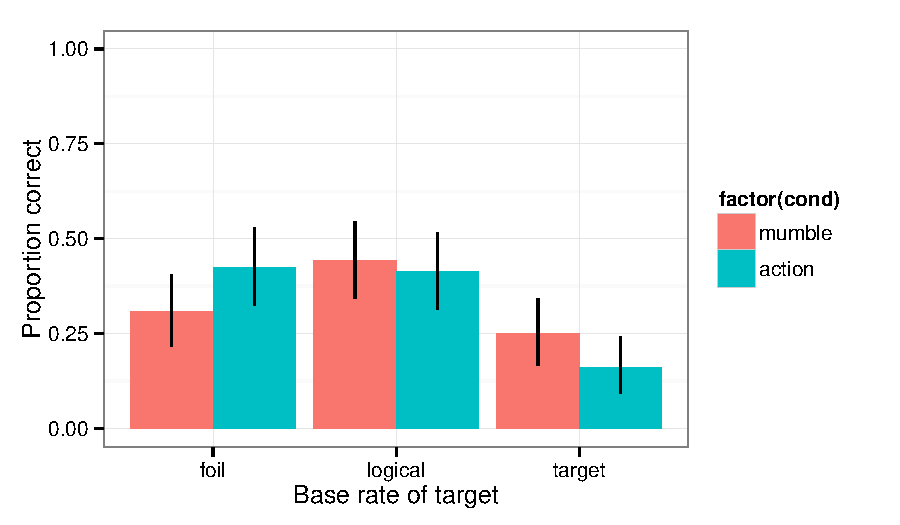
\includegraphics[width=5in]{../plots/2-prior-frame.pdf}
  \caption{\label{fig:prelims-dv} Data from \exptref{exp:prior-frame}. Colors indicate different methods for eliciting prior expectations.}
\end{figure}

In \exptref{exp:prior-frame}, we compared prior elicitation methods. We presented participants with the same canonical display we had used in the prior experiments, but asked them one of two prior questions. The reference prior method was based on \citeA{frank2012}, where the participant was told that ``Bob can say one word'' but the word was presented as ``mumblemumble (you didn't hear what he said).'' The action prior method consisted of simply asking, e.g. ``Which friend do you think Bob will visit next?'' The distribution of responses did not differ between the two questions ($\chi^2(2) = 3.45,~p = .18$, Figure \ref{fig:prior-frame}). Overall, participants showed a tendency to choose the logical target (e.g., face with both hat and glasses) most, the foil at intermediate rates, and the pragmatic target relatively less. While this experiment is not decisive regarding the underlying philosophical issue of what kinds of expectations the prior actually tracks, we put aside this issue for the time being and adopt the mumble prior elicitation method for subsequent experiments (as the choice does not appear critical for our purposes).

\begin{figure}[t]
  \centering
  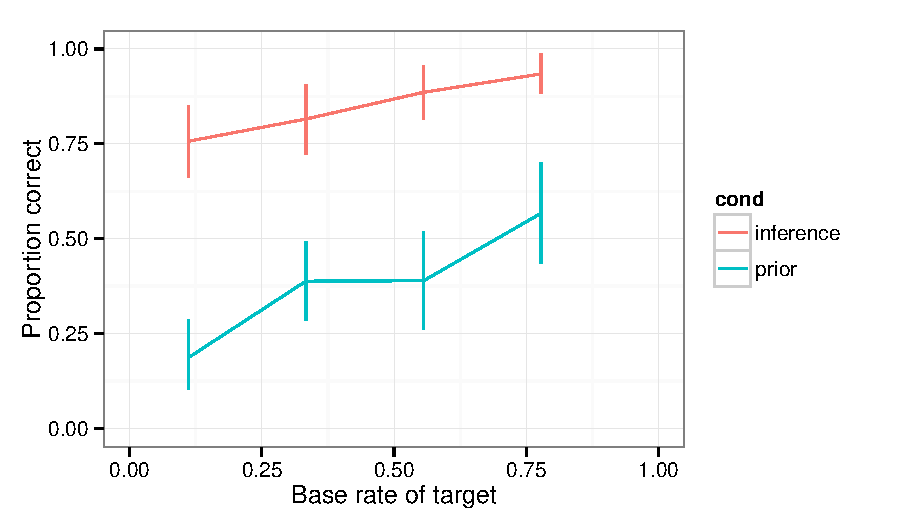
\includegraphics[width=5in]{../plots/2-prior-baserates.pdf}
  \caption{\label{fig:prior-baserate} Data from \exptref{exp:prior-baserates} from prior elicitation and inference conditions. Horizontal axis shows the proportion of familiarization trials that showed the target.}
\end{figure}

In \exptref{expt:baserate}, we attempted to manipulate participants' prior expectations about reference via a manipulation of the base rate of the interlocutor's actions.\footnote{This experiment is conceptually similar to a base-rate manipulation reported in \citeA{stiller2011}. Note however that the manipulation in that experiment uses a different display, one more similar to those used in \exptref{exp:levels-level}.} Prior to showing the target inference, we exposed participants to evidence about the habits of the interlocutor (Bob). The familiarization screen in this experiment stated (for example, in the case of the face stimulus) that Bob visited a friend every week; it then invited the participant to click on nine boxes to uncover the nine friends that Bob had visited most recently. Across four base rate conditions, we manipulated how many of these boxes contained the pragmatic target (e.g., the face with glasses and no hat). One of the boxes always contained the foil (no glasses or hat) and another contained the logical target (hat and glasses). Then the other boxes contained either the pragmatic or the logical target. The four conditions were created such that 1/9, 3/9, 5/9, and 7/9 boxes showed the pragmatic target. 

Figure \ref{fig:prior-baserate} shows the results of this manipulation.\footnote{This experiment had unusually high rates of exclusion due to participants' confusion about whether they should report  familiarization frequencies for the manipulation check. We maintain our strict inclusion criterion here but note that the results are largely unchanged if we include these participants.}  The base rate had a strong effect on the prior elicitation, but it also boosted levels of pragmatic inferences. To quantify these effects preliminary to model fitting, we used a logistic regression model (no hierarchical model was warranted because judgments are from independent participants). This model showed highly significant effects of base rate ($\beta = .27,~p = .004$) and condition  (with prior as the dummy-coded predictor, $\beta = -.57,~p < .0001$), as well as a marginal interaction of the two  ($\beta = .29,~p = .06$). Critically, the main effect of base rate remained reliable in a similar logistic regression for just the inference trials ($\beta = .28,~p = .0001$), indicating a highly reliable (and graded) effect of the base-rate manipulation on the strength of the pragmatic inference.


\begin{figure}[t]
  \centering
  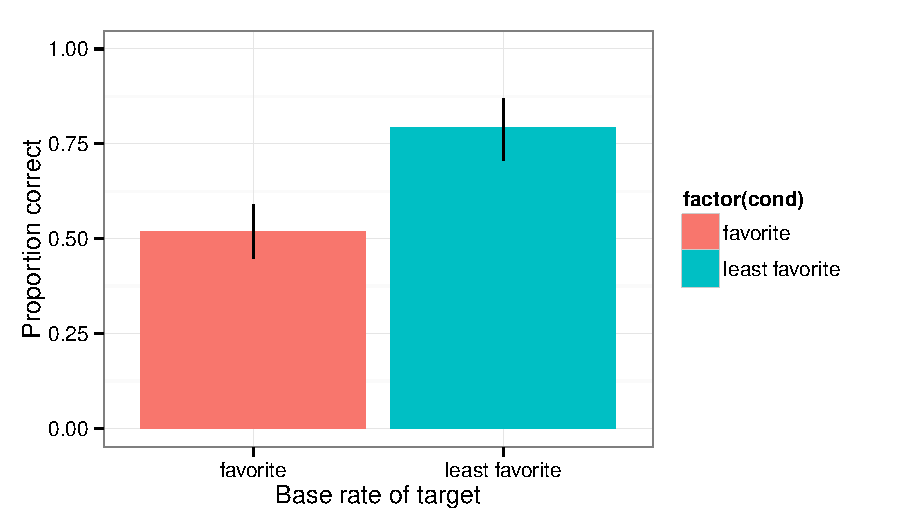
\includegraphics[width=4in]{../plots/2-prior-valence.pdf}
  \caption{\label{fig:prior-valence} Data from \exptref{exp:prior-valence} in the inference conditions.}
\end{figure}

Our next experiment, \exptref{exp:prior-valence}, investigated the effects of linguistic manipulations on participants' priors and their resulting inferences. In this experiment, we framed judgments as being about determining Bob's \emph{favorite} or \emph{least favorite} item.\footnote{This experiment had four items: faces, boats, pizzas, and snowmen.'} We reasoned that, all else being equal, his favorite item would likely have more features, while his least favorite friend would likely have more. Prior measurements supported this conclusion: The logical option, which had the most features, was chosen as ``favorite'' 70\% of the time, while the distractor option, which had zero features, was chosen as ``least favorite'' 77\% of the time. Pragmatic inferences reflected these changing expectations, with participants far less likely to choose the pragmatic target in the inference condition with a ``favorite'' frame than with a ``least favorite'' frame (Figure \ref{fig:prior-valence}).  


\begin{figure}[t]
  \centering
  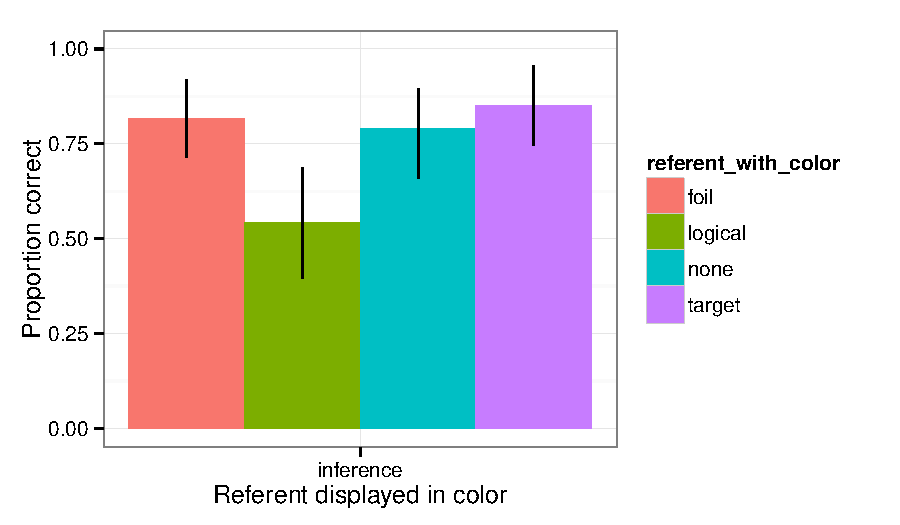
\includegraphics[width=4in]{../plots/2-prior-color.pdf}
  \caption{\label{fig:prior-color} Data from \exptref{exp:prior-color} in the inference conditions.}
\end{figure}

Our final experiment in this sequence, \exptref{exp:prior-color}, attempted to manipulate prior expectations about reference by changing the salience of the different referents. In particular, we presented all but one of the images in grayscale, varying which of the images (pragmatic target, logical target, or foil) was shown in color.\footnote{To ensure that participants still made the inference more generally, we included a condition where none of the referents was shown in color, notated by ``none.''} This manipulation had a strong effect on both prior expectations and pragmatic inferences. In particular, when the logical target was shown in color, inferences to the pragmatic target dropped substantially (Figure \ref{fig:prior-color}). 

In sum, Experiments \exptrefrange{exp:prior-baserate}{exp:prior-color} show strong evidence that a variety of manipulations can affect prior expectations about reference. In \secref{sec:models}, we return to these data and test the stronger hypothesis that variation in inference levels in these three experiments can be accounted for by variation in prior expectations. 
 